% Provenance (never printed): cycle 4 SVT/physique, "La planete Terre,
% l'environnement": the ocean, its relief, its waters and their movements;
% see sources/book1/PROVENANCE.md. Book 1, grade 8, chapter 4.
% Vocabulary guard: owns the parts of the seafloor (one definition),
% salinity, ocean current (homograph: electric current -- link "ocean
% current" only), gyre. Ridge and trench were met as places in g7.1 (plate
% boundaries); seafloor spreading and subduction stay there. The deep
% circulation is told (no "thermohaline" definition: Book 2).
\chapter{Les océans}\label{ch:g8:the-oceans}

En décembre 1872, un navire de la marine britannique, le HMS
\emph{Challenger}, quitta l'Angleterre pour un voyage de trois ans et demi
autour du monde. Sa mission était nouvelle~: découvrir ce qui se trouve au
fond des \omterm{def:g2:water-on-earth:ocean}{océans}. Encore et encore, le navire s'arrêtait en pleine \omterm{def:g2:water-on-earth:ocean}{mer}, et
l'équipage descendait un lourd poids au bout d'une longue corde jusqu'à ce
qu'il touche le fond~; la longueur de corde déroulée donnait la profondeur.
Quand le navire rentra, en mai 1876, ses sondages avaient montré que le fond de l'\omterm{def:g2:water-on-earth:ocean}{océan}
a des \omterm{def:g1:landscapes-around-us:landform}{plaines} profondes et de grandes \omterm{def:g4:world-physical-map:range}{chaînes de montagnes}.
% ledger: nhm:challenger-voyage, edin:challenger-stations

\begin{omfigure}
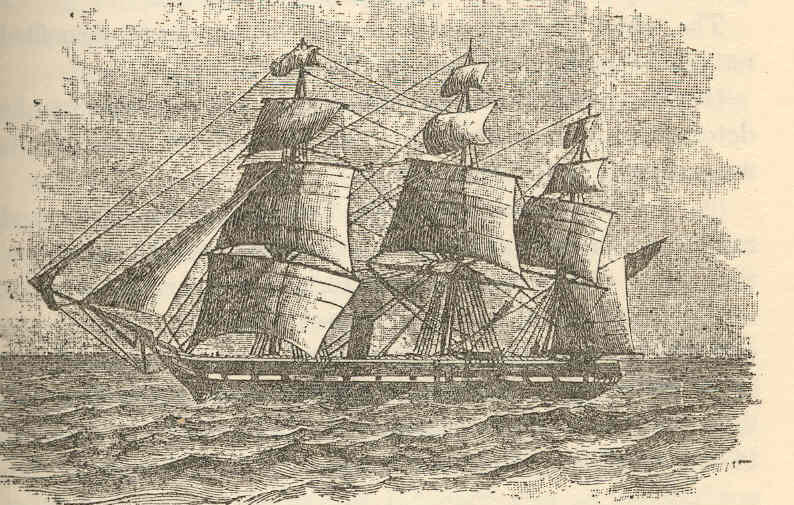
\includegraphics[width=0.55\linewidth]{images/book1/g8-challenger-sounding.jpg}

{\small Le HMS \emph{Challenger} se prépare à sonder la profondeur de
l'\omterm{def:g2:water-on-earth:ocean}{océan}, 1872. Gravure tirée des rapports de l'expédition, reproduite dans
W.~A.~Herdman, \emph{Founders of Oceanography} (1923)~; domaine public, via
Wikimedia Commons.}
% ledger: commons:challenger
\label{fig:g8:the-oceans:challenger}
\end{omfigure}

Aujourd'hui, un navire cartographie le fond de la \omterm{def:g2:water-on-earth:ocean}{mer} avec le son. Un
appareil placé sous sa coque envoie vers le bas une brève impulsion
sonore~; le son rebondit sur le fond et revient sous forme d'écho. Le
temps que met l'écho donne la profondeur, encore et encore, pendant que le
navire continue d'avancer. C'est le \emph{sonar}.
% ledger: nos:sonar

\begin{recall}
L'\omterm{def:g2:water-on-earth:salt-fresh}{eau salée} couvre la plus grande partie de la Terre, en un seul \omterm{def:g2:water-on-earth:ocean}{océan}
mondial divisé en \omterm{def:g2:water-on-earth:ocean}{océans} et en \omterm{def:g2:water-on-earth:ocean}{mers} (\cref{ch:g2:water-on-earth}). Les
\omterm{def:g7:plate-tectonics:plate}{plaques} s'écartent au niveau des \omterm{def:g8:the-oceans:seafloor}{dorsales océaniques}, et une \omterm{def:g7:plate-tectonics:plate}{plaque}
s'enfonce sous une autre au niveau des fosses
(\cref{ch:g7:plate-tectonics}). Au-dessus des \omterm{def:g2:water-on-earth:ocean}{océans}, les vents soufflent
en grandes bandes~: \omterm{def:g8:winds-global-circulation:global-winds}{alizés}, \omterm{def:g8:winds-global-circulation:global-winds}{vents d'ouest} et \omterm{def:g8:winds-global-circulation:global-winds}{vents d'est polaires}, déviés
par la rotation de la Terre (\cref{ch:g8:winds-global-circulation}).
\end{recall}

\section{Le fond de l'océan}

Si l'on pouvait vider l'eau des \omterm{def:g2:water-on-earth:ocean}{océans}, tout un \omterm{def:g1:landscapes-around-us:landscape}{paysage} caché
apparaîtrait. Le long des \omterm{def:g1:landscapes-around-us:water}{côtes}, la terre se prolonge sous la \omterm{def:g2:water-on-earth:ocean}{mer} par un
plateau peu profond, en pente douce. Puis le fond plonge par une pente
raide jusqu'à de vastes \omterm{def:g1:landscapes-around-us:landform}{plaines} plates, à des kilomètres de profondeur. Des
\omterm{def:g4:world-physical-map:range}{chaînes de montagnes} s'élèvent de ces \omterm{def:g1:landscapes-around-us:landform}{plaines}, et çà et là d'étroites
fosses descendent plus bas que tout autre endroit de la Terre.
% ledger: edin:challenger-stations

\begin{omfigure}
\begin{tikzpicture}[font=\footnotesize, >={Stealth[length=2mm]}]
  \fill[omSea] (0,0) rectangle (15.6,-4.2);
  \fill[omLithAlluv] (0,0.6) -- (1.2,0.15) -- (1.6,0) -- (3.4,-0.35)
    .. controls (3.9,-0.55) and (4.1,-2.6) .. (4.7,-3.1)
    -- (6.6,-3.35) -- (7.6,-3.1) -- (8.3,-2.2) -- (8.6,-1.7) -- (8.75,-1.9) -- (8.9,-1.65) -- (9.2,-2.3) -- (10.0,-3.15)
    -- (11.6,-3.4) -- (12.6,-3.45) -- (13.05,-4.1) -- (13.35,-3.0) -- (14.2,-0.9) -- (14.8,0.7) -- (15.6,1.3)
    -- (15.6,-4.6) -- (0,-4.6) -- cycle;
  \draw[black!70] (0,0.6) -- (1.2,0.15) -- (1.6,0) -- (3.4,-0.35)
    .. controls (3.9,-0.55) and (4.1,-2.6) .. (4.7,-3.1)
    -- (6.6,-3.35) -- (7.6,-3.1) -- (8.3,-2.2) -- (8.6,-1.7) -- (8.75,-1.9) -- (8.9,-1.65) -- (9.2,-2.3) -- (10.0,-3.15)
    -- (11.6,-3.4) -- (12.6,-3.45) -- (13.05,-4.1) -- (13.35,-3.0) -- (14.2,-0.9) -- (14.8,0.7) -- (15.6,1.3);
  \draw[omRiver] (1.55,0) -- (14.45,0);
  \node[anchor=south] at (8,0.05) {niveau de la mer};
  \node[align=center] at (2.6,-0.85) {plateau\\continental};
  \draw[->] (2.6,-0.55) -- (2.6,-0.25);
  \node[align=center, anchor=east] at (3.7,-2.0) {talus\\continental};
  \draw[->] (3.75,-2.0) -- (4.1,-1.9);
  \node[align=center] at (5.7,-2.6) {plaine abyssale};
  \node[align=center] at (8.75,-0.9) {dorsale océanique};
  \draw[->] (8.75,-1.15) -- (8.75,-1.55);
  \node[align=center] at (11.1,-2.6) {plaine abyssale};
  \node[align=center, anchor=west] at (13.5,-3.9) {fosse\\océanique};
  \draw[->] (13.45,-3.9) -- (13.15,-3.9);
  \node[anchor=south] at (0.8,0.6) {continent};
  \node[anchor=south east] at (14.7,1.0) {montagnes};
\end{tikzpicture}

{\small Les parties du fond de l'\omterm{def:g2:water-on-earth:ocean}{océan}, d'une \omterm{def:g1:landscapes-around-us:water}{côte} jusqu'au large et
jusqu'à une autre \omterm{def:g1:landscapes-around-us:water}{côte} (un croquis~: les profondeurs et les largeurs ne
sont pas à l'échelle).}
\label{fig:g8:the-oceans:sketch}
\end{omfigure}

\begin{definition}[Les parties du fond de l'océan]\label{def:g8:the-oceans:seafloor}
\begin{itemize}
  \item Le \emph{plateau continental}\index{plateau continental} est le
        bord d'un \omterm{def:g3:continents-and-oceans:continent}{continent} sous la \omterm{def:g2:water-on-earth:ocean}{mer}, peu profond et en pente douce.
  \item Le \emph{talus continental}\index{talus continental} est la pente
        raide qui descend du plateau jusqu'au fond de l'\omterm{def:g2:water-on-earth:ocean}{océan} profond.
  \item Une \emph{plaine abyssale}\index{plaine abyssale} est une partie
        vaste, très plate et profonde du fond de l'\omterm{def:g2:water-on-earth:ocean}{océan}.
  \item Une \emph{dorsale océanique}\index{dorsale oceanique@dorsale océanique}
        est une longue \omterm{def:g4:world-physical-map:range}{chaîne de montagnes} sous-marines qui s'élève des
        \omterm{def:g1:landscapes-around-us:landform}{plaines} abyssales.
  \item Une \emph{fosse océanique}\index{fosse oceanique@fosse océanique}
        est un sillon long, étroit et très profond du fond de l'\omterm{def:g2:water-on-earth:ocean}{océan},
        souvent voisin d'une \omterm{def:g4:world-physical-map:range}{chaîne de montagnes} ou d'îles volcaniques.
\end{itemize}
\end{definition}
% ledger: edin:challenger-stations, usgs:trench-depth

L'\omterm{def:g2:water-on-earth:ocean}{océan} a une profondeur moyenne d'environ \qty{3700}{m}, presque la
moitié de la hauteur de la plus haute \omterm{def:g1:landscapes-around-us:landform}{montagne} des terres émergées. Son
point le plus profond, la fosse Challenger, dans la fosse des Mariannes, dans
l'\omterm{def:g2:water-on-earth:ocean}{océan} Pacifique, se trouve à près de \qty{11000}{m} sous la surface.
% ledger: nos:ocean-depth, usgs:trench-depth, tht:everest


\begin{method}[Lire un profil du fond de l'océan]
\begin{enumerate}
  \item Lis les axes~: la distance d'un côté à l'autre, la hauteur ou la
        profondeur de haut en bas, et l'exagération verticale.
  \item Trouve le \omterm{def:g4:world-physical-map:altitude}{niveau de la mer} (hauteur 0) et les \omterm{def:g1:landscapes-around-us:water}{côtes}, là où le
        profil le traverse.
  \item Suis le fond à partir d'une \omterm{def:g1:landscapes-around-us:water}{côte}~: le plateau peu profond, la pente
        raide, puis les \omterm{def:g1:landscapes-around-us:landform}{plaines} profondes et plates.
  \item Cherche ce qui s'élève au-dessus des \omterm{def:g1:landscapes-around-us:landform}{plaines} (une dorsale) ou
        descend au-dessous (une fosse), et lis sa profondeur.
\end{enumerate}
\end{method}

\begin{example}[À travers l'Atlantique Sud]
Sur le profil du haut, après la \omterm{def:g1:landscapes-around-us:water}{côte} de l'Amérique du Sud, le fond
descend à plus de \qty{3000}{m} de profondeur en moins de \qty{300}{km}. Des \omterm{def:g8:the-oceans:seafloor}{plaines abyssales},
entre \qty{3500}{m} et \qty{5000}{m} de profondeur, occupent la plus grande
partie de la largeur. À mi-chemin, à environ \qty{4400}{km} le long du
profil, la dorsale médio-atlantique s'élève jusqu'à environ \qty{2300}{m}
sous la surface~: plus de \qty{2000}{m} au-dessus des \omterm{def:g1:landscapes-around-us:landform}{plaines}, une \omterm{def:g4:world-physical-map:range}{chaîne
de montagnes} cachée sous la \omterm{def:g2:water-on-earth:ocean}{mer}. Les \omterm{def:g1:landscapes-around-us:landform}{plaines} redescendent à plus de
\qty{5000}{m} avant que le fond ne remonte vers l'Afrique.
\end{example}
% ledger: data:etopo1 (figdata/grade-8/seafloor_profile.py: ridge crest -2329 m at 4407 km; deepest -5295 m)

\begin{omfigure}
\begin{tikzpicture}
\begin{axis}[omsection, scale only axis, width=14cm, height=3.6cm, xmin=0, xmax=7569,
  ymin=-6000, ymax=1500, ytick={-6000,-4000,-2000,0}, xtick={0,1000,...,7000},
  xlabel={distance le long de 30.5\textdegree\ S, depuis 59.5\textdegree\ O (km)}, ylabel={altitude (m)},
  tick label style={font=\scriptsize}, label style={font=\small},
  yticklabel style={/pgf/number format/1000 sep={\,}}, xticklabel style={/pgf/number format/1000 sep={\,}},
  axis background/.style={fill=white}, clip=true]
  \fill[omSea] (axis cs:0,-6000) rectangle (axis cs:7569,0);
  \addplot[fill=omLithAlluv, draw=black!70, line width=0.5pt] table[x=km, y=elev_m] {figdata/out/grade-8-seafloor_profile-atlantic-rock.dat};
  \node[font=\scriptsize, align=center, fill=white, inner sep=1pt] at (axis cs:4407,-900) {dorsale médio-atlantique};
  \draw[-{Stealth[length=1.5mm]}] (axis cs:4407,-1250) -- (axis cs:4407,-2150);
  \node[font=\scriptsize] at (axis cs:2500,-5300) {plaine abyssale};
  \node[font=\scriptsize] at (axis cs:6200,-5600) {plaine abyssale};
  \node[font=\scriptsize, anchor=south west] at (axis cs:30,350) {Amérique du Sud};
  \node[font=\scriptsize, anchor=south east] at (axis cs:7380,350) {Afrique};
  \node[anchor=north] at (rel axis cs:0.75,0.97) {\omve{260}};
\end{axis}
\end{tikzpicture}

\medskip
\begin{tikzpicture}
\begin{axis}[omsection, scale only axis, width=7cm, height=3.6cm, xmin=0, xmax=3020,
  ymin=-6000, ymax=4500, ytick={-6000,-4000,-2000,0,2000,4000}, xtick={0,1000,2000,3000},
  xlabel={distance le long de 20.5\textdegree\ S (km)}, ylabel={altitude (m)},
  tick label style={font=\scriptsize}, label style={font=\small},
  yticklabel style={/pgf/number format/1000 sep={\,}}, xticklabel style={/pgf/number format/1000 sep={\,}},
  axis background/.style={fill=white}, clip=true]
  \fill[omSea] (axis cs:0,-6000) rectangle (axis cs:3020,0);
  \addplot[fill=omLithAlluv, draw=black!70, line width=0.5pt] table[x=km, y=elev_m] {figdata/out/grade-8-seafloor_profile-pacific-rock.dat};
  \node[font=\scriptsize, align=center, fill=white, inner sep=1pt] at (axis cs:1300,1600) {fosse du Pérou--Chili};
  \draw[-{Stealth[length=1.5mm]}] (axis cs:1750,1150) -- (axis cs:1870,-5000);
  \node[font=\scriptsize, anchor=west] at (axis cs:2600,3500) {Andes};
  \node[font=\scriptsize] at (axis cs:700,-5300) {plaine abyssale};
  \node[anchor=north west] at (rel axis cs:0.01,0.98) {\omve{148}};
\end{axis}
\end{tikzpicture}

{\small Deux profils réels du fond de l'\omterm{def:g2:water-on-earth:ocean}{océan}, tirés du relief ETOPO1 lu
à chaque degré de \omterm{def:g6:latitude-longitude:longitude}{longitude}. En haut~: à travers l'Atlantique Sud, de
l'Amérique du Sud à l'Afrique. En bas~: à travers la bordure pacifique de
l'Amérique du Sud. Les hauteurs sont étirées 260 et 148~fois par rapport
aux distances (\emph{exagération verticale}), sans quoi l'\omterm{def:g2:water-on-earth:ocean}{océan} paraîtrait
aussi mince qu'une feuille de papier~; et avec un point par degré, la
fosse étroite paraît moins profonde qu'elle ne l'est.}
% ledger: data:etopo1, earth:Rmean (figdata/grade-8/seafloor_profile.py)
\label{fig:g8:the-oceans:profiles}
\end{omfigure}


\section{Une eau salée}

L'eau de \omterm{def:g2:water-on-earth:ocean}{mer} a un goût salé parce que des sels y sont dissous. La plupart
viennent des \omterm{def:g3:stones-pebbles-sand:rock}{roches} des \omterm{def:g3:continents-and-oceans:continent}{continents}~: la \omterm{def:g4:clouds-rain-snow:precipitation}{pluie} use lentement les \omterm{def:g3:stones-pebbles-sand:rock}{roches}, et
les \omterm{def:g1:landscapes-around-us:water}{rivières} apportent leurs sels dissous à la \omterm{def:g2:water-on-earth:ocean}{mer}. Certains viennent de
sources chaudes du fond de l'\omterm{def:g2:water-on-earth:ocean}{océan}.
% ledger: nos:salinity-varies

\begin{definition}[Salinité]\label{def:g8:the-oceans:salinity}
La \emph{salinité}\index{salinite@salinité} de l'eau de \omterm{def:g2:water-on-earth:ocean}{mer} est la masse de
sels dissous dans un kilogramme d'eau de \omterm{def:g2:water-on-earth:ocean}{mer}. En moyenne, elle est
d'environ \qty{35}{g} par kilogramme~: \qty{3.5}{\%} de la masse de l'eau
de \omterm{def:g2:water-on-earth:ocean}{mer} est du sel.
\end{definition}
% ledger: nos:salinity-varies

La \omterm{def:g8:the-oceans:salinity}{salinité} n'est pas la même partout. Quand l'eau de \omterm{def:g2:water-on-earth:ocean}{mer} s'évapore, l'eau
s'en va mais les sels restent~: là où le Soleil est fort et la \omterm{def:g4:clouds-rain-snow:precipitation}{pluie} rare,
la \omterm{def:g2:water-on-earth:ocean}{mer} devient plus salée. Là où il tombe beaucoup de \omterm{def:g4:clouds-rain-snow:precipitation}{pluie}, ou là où se
jette un grand fleuve, la \omterm{def:g2:water-on-earth:ocean}{mer} est moins salée. Quand l'eau de \omterm{def:g2:water-on-earth:ocean}{mer} gèle en
banquise, le sel reste dans l'eau autour, qui devient elle aussi plus
salée. Dans l'ensemble, la \omterm{def:g8:the-oceans:salinity}{salinité} est faible près de l'\omterm{def:g3:continents-and-oceans:equator}{équateur}, où il
pleut beaucoup, et près des \omterm{def:g3:continents-and-oceans:poles}{pôles}~; elle est la plus forte aux \omterm{def:g6:latitude-longitude:latitude}{latitudes}
moyennes, sous les bandes sèches situées vers \ang{30}.
% ledger: nos:salinity-varies, nos:sea-ice-salt, mo:three-cells

\begin{omfigure}
\begin{tikzpicture}[font=\footnotesize, >={Stealth[length=2mm]}]
  \fill[omSea] (0,0) rectangle (13,-1.6);
  \draw[omRiver, line width=0.8pt] (0,0) -- (13,0);
  % left: dry belt, evaporation
  \fill[yellow!80!orange] (1.2,3.0) circle (0.35);
  \foreach \x in {1.0,1.8,2.6,3.4} \draw[->, black!50, line width=0.9pt, decorate, decoration={snake, amplitude=0.6mm, segment length=3mm}] (\x,0.15) -- (\x,1.6);
  \node[align=center] at (2.3,2.2) {forte évaporation,\\peu de pluie};
  \node[align=center, fill=white, inner sep=1.5pt] at (2.3,-0.8) {\textbf{plus salée}};
  % middle: rain
  \fill[black!20] (5.2,2.9) ellipse [x radius=1.3, y radius=0.4];
  \foreach \x in {4.4,4.8,...,6.0} \draw[omRiver] (\x,2.45) -- (\x-0.2,0.25);
  \node[align=center, fill=white, inner sep=1.5pt] at (5.2,-0.8) {\textbf{moins salée}};
  \node at (5.2,3.55) {fortes pluies};
  % right: river mouth and sea ice
  \fill[omLithAlluv] (7.4,0) -- (9.6,0) -- (9.6,0.6) -- (7.4,0.35) -- cycle;
  \draw[omRiver, line width=2pt, ->] (9.4,0.45) -- (7.9,0.2);
  \node[anchor=south] at (8.6,0.65) {fleuve};
  \node[align=center, fill=white, inner sep=1.5pt] at (8.6,-0.8) {\textbf{moins salée}};
  \fill[white, draw=omCold] (10.6,0.25) -- (12.6,0.25) -- (12.4,-0.25) -- (10.8,-0.25) -- cycle;
  \node[anchor=south] at (11.6,0.3) {la banquise se forme};
  \node[align=center, fill=white, inner sep=1.5pt] at (11.6,-0.95) {\textbf{plus salée}\\(le sel reste)};
\end{tikzpicture}

{\small Ce qui change la \omterm{def:g8:the-oceans:salinity}{salinité} de la \omterm{def:g2:water-on-earth:ocean}{mer}~: l'évaporation et le gel
laissent les sels derrière eux~; la \omterm{def:g4:clouds-rain-snow:precipitation}{pluie} et les fleuves apportent de
l'\omterm{def:g2:water-on-earth:salt-fresh}{eau douce}.}
% ledger: nos:salinity-varies, nos:sea-ice-salt
\label{fig:g8:the-oceans:salinity}
\end{omfigure}

\begin{omfigure}
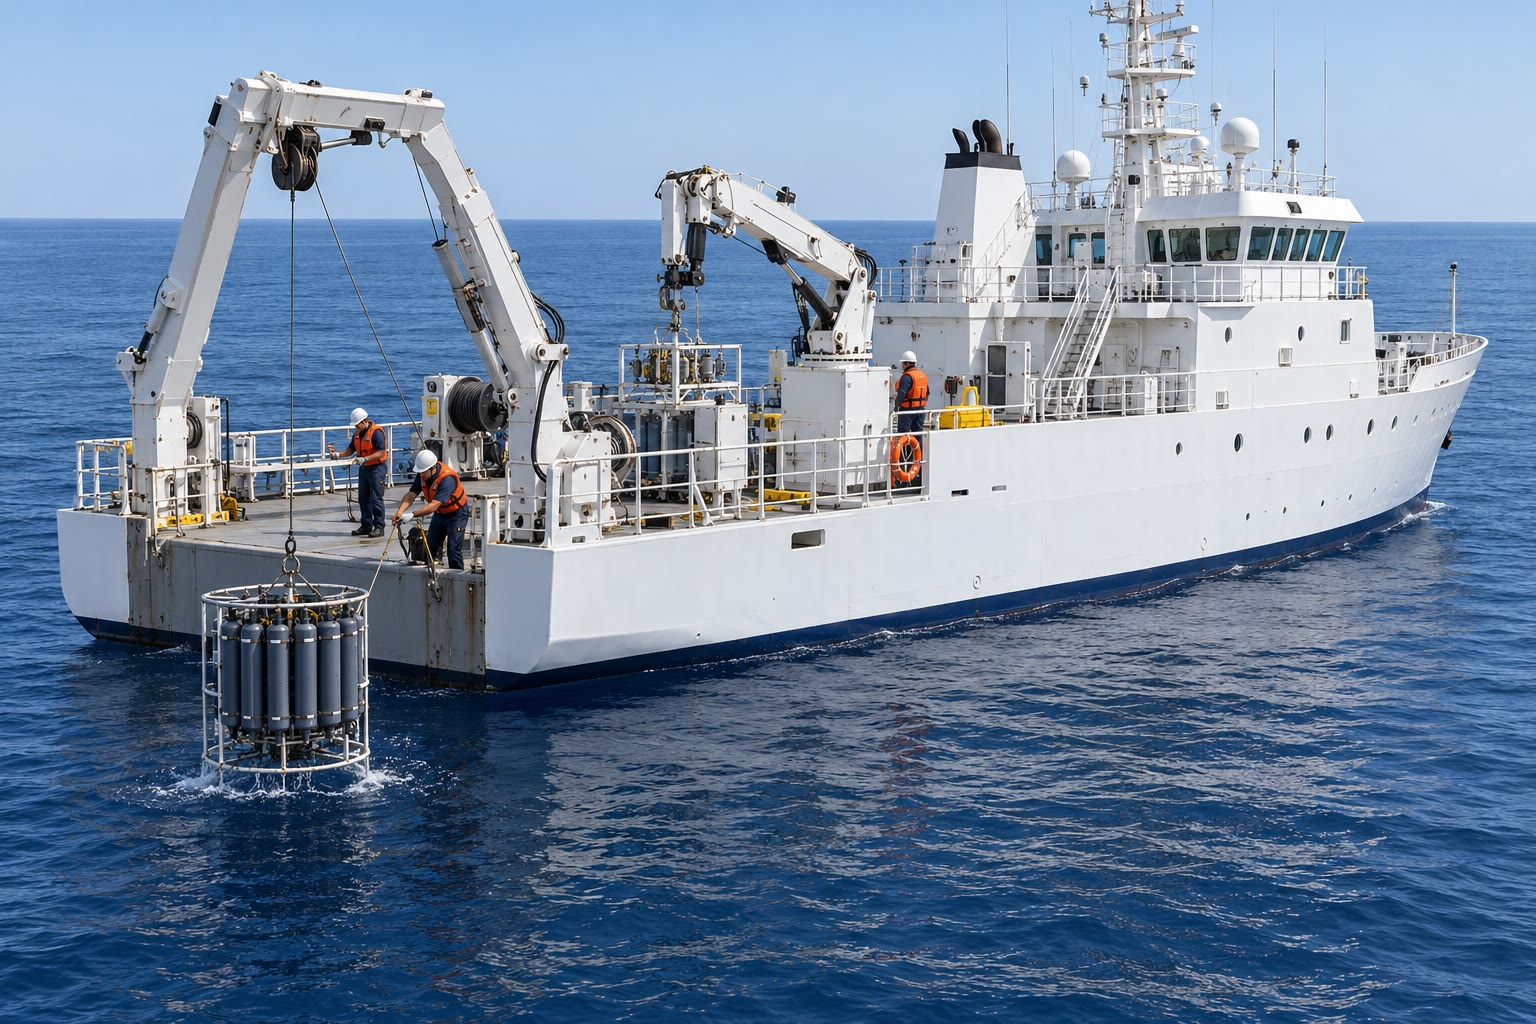
\includegraphics[width=0.58\linewidth]{images/book1/ai/g8-research-ship.jpg}

{\small Un navire de recherche descend dans la \omterm{def:g2:water-on-earth:ocean}{mer} un cadre de bouteilles
de prélèvement, pour rapporter de l'eau des profondeurs et mesurer sa
\omterm{def:g8:the-oceans:salinity}{salinité} et sa température (illustration générée par IA d'une scène
générique).}
\label{fig:g8:the-oceans:ship}
\end{omfigure}

\section{Les courants de surface}

L'\omterm{def:g2:water-on-earth:ocean}{océan} n'est jamais immobile. Les vents frottent sur sa surface et mettent
l'eau en mouvement~: les \omterm{def:g8:winds-global-circulation:global-winds}{alizés} réguliers la poussent vers l'ouest près de
l'\omterm{def:g3:continents-and-oceans:equator}{équateur}, et les \omterm{def:g8:winds-global-circulation:global-winds}{vents d'ouest} la poussent vers l'est aux \omterm{def:g6:latitude-longitude:latitude}{latitudes}
moyennes. Comme les vents, l'eau en mouvement est déviée par la rotation
de la Terre~: vers la droite dans l'\omterm{def:g3:continents-and-oceans:equator}{hémisphère} Nord, vers la gauche dans
l'\omterm{def:g3:continents-and-oceans:equator}{hémisphère} Sud.
% ledger: nos:gyres

\begin{definition}[Courant océanique et gyre]\label{def:g8:the-oceans:current}
Un \emph{courant océanique}\index{courant oceanique@courant océanique} est
un mouvement régulier de l'eau de \omterm{def:g2:water-on-earth:ocean}{mer} dans une direction, comme un fleuve
dans l'\omterm{def:g2:water-on-earth:ocean}{océan}. Un \emph{gyre}\index{gyre} est une très grande boucle de
courants océaniques qui tourne autour d'un bassin océanique.
\end{definition}
% ledger: nos:gyre-def, nos:gyres
\phantomsection\label{def:g8:the-oceans:gyre}

Il y a cinq grands \omterm{def:g8:the-oceans:current}{gyres}~: dans l'Atlantique Nord et Sud, dans le
Pacifique Nord et Sud, et dans l'\omterm{def:g2:water-on-earth:ocean}{océan} Indien. Ceux de l'\omterm{def:g3:continents-and-oceans:equator}{hémisphère} Nord
tournent dans le sens des aiguilles d'une montre, ceux de l'\omterm{def:g3:continents-and-oceans:equator}{hémisphère} Sud
dans le sens inverse. Sur le côté ouest de chaque \omterm{def:g2:water-on-earth:ocean}{océan}, le courant du
\omterm{def:g8:the-oceans:current}{gyre} est étroit et rapide~; sur le côté est, il est large et lent.
% ledger: nos:gyres

\begin{inthelab}[Un gyre dans un plat]
À l'intérieur, remplis d'eau un grand plat rond et saupoudre la surface
d'une pincée de poivre. Souffle doucement et régulièrement à travers une
paille au-dessus du plat, toujours dans la même direction, près d'un bord.
Observe le poivre~: l'eau de surface se met à bouger avec ton souffle, et
bientôt toute la surface tourne en boucle dans le plat.
\end{inthelab}

\begin{omfigure}
\begin{tikzpicture}
\begin{axis}[ommap, width=\linewidth, xmin=-180, xmax=180, ymin=-65, ymax=70,
  xtick={-180,-120,...,180}, ytick={-60,-30,0,30,60},
  xticklabels={$180^\circ$,$120^\circ$O,$60^\circ$O,$0^\circ$,$60^\circ$E,$120^\circ$E,$180^\circ$},
  yticklabels={$60^\circ$S,$30^\circ$S,$0^\circ$,$30^\circ$N,$60^\circ$N},
  tick label style={font=\scriptsize}]
  \addplot[fill=omLithAlluv, draw=black!45, line width=0.2pt] table {figdata/out/shared-geo-land.dat};
  \addplot[omWarm, line width=1.3pt] table {figdata/out/grade-8-ocean_currents-gyres-warm.dat};
  \addplot[omCold, line width=1.3pt] table {figdata/out/grade-8-ocean_currents-gyres-cold.dat};
  \addplot[quiver={u=\thisrow{u}, v=\thisrow{v}}, -{Stealth[length=2.6mm, width=2.2mm]}, omWarm, line width=1.3pt]
    table[x=lon, y=lat] {figdata/out/grade-8-ocean_currents-heads-warm.dat};
  \addplot[quiver={u=\thisrow{u}, v=\thisrow{v}}, -{Stealth[length=2.6mm, width=2.2mm]}, omCold, line width=1.3pt]
    table[x=lon, y=lat] {figdata/out/grade-8-ocean_currents-heads-cold.dat};
  \node[font=\scriptsize\bfseries, fill=white, inner sep=1pt, anchor=east] at (axis cs:-72,40) {Gulf Stream};
  \node[font=\scriptsize\bfseries, fill=white, inner sep=1pt, anchor=west] at (axis cs:-12,25) {C. des Canaries};
\end{axis}
\end{tikzpicture}

{\small Les cinq grands \omterm{def:g8:the-oceans:current}{gyres}, simplifiés~: dans le sens des aiguilles
d'une montre dans l'\omterm{def:g3:continents-and-oceans:equator}{hémisphère} Nord, dans le sens inverse dans
l'\omterm{def:g3:continents-and-oceans:equator}{hémisphère} Sud. En rouge~: les courants chauds, venus des \omterm{def:g5:weather-and-climate:tropics}{tropiques}~; en
bleu~: les courants froids, venus de plus hautes \omterm{def:g6:latitude-longitude:latitude}{latitudes}. Le \omterm{def:g8:the-oceans:current}{gyre} de
l'Atlantique Nord est bordé par le Gulf Stream à l'ouest et par le courant
des Canaries à l'est.}
% ledger: nos:gyres, data:ne-land (figdata/grade-8/ocean_currents.py)
\label{fig:g8:the-oceans:gyres}
\end{omfigure}

Le plus connu de ces courants est le Gulf Stream. Il sort du golfe du
Mexique, remonte vers le nord le long de la \omterm{def:g1:landscapes-around-us:water}{côte} de la Floride, tourne
vers l'est au large de la Caroline du Nord et traverse l'Atlantique vers
le nord-est. Son eau chaude avance en moyenne à environ \qty{6.4}{km} par
heure, jusqu'à environ \qty{9}{km} par heure en surface, et il transporte
plus d'eau que tous les fleuves du monde réunis. Il garde la \omterm{def:g1:landscapes-around-us:water}{côte} est de
la Floride plus chaude en hiver et apporte un air doux à l'Europe de
l'Ouest.
% ledger: nos:gulf-stream, nos:gyres

\begin{omfigure}
\begin{minipage}[c]{0.5\linewidth}\centering
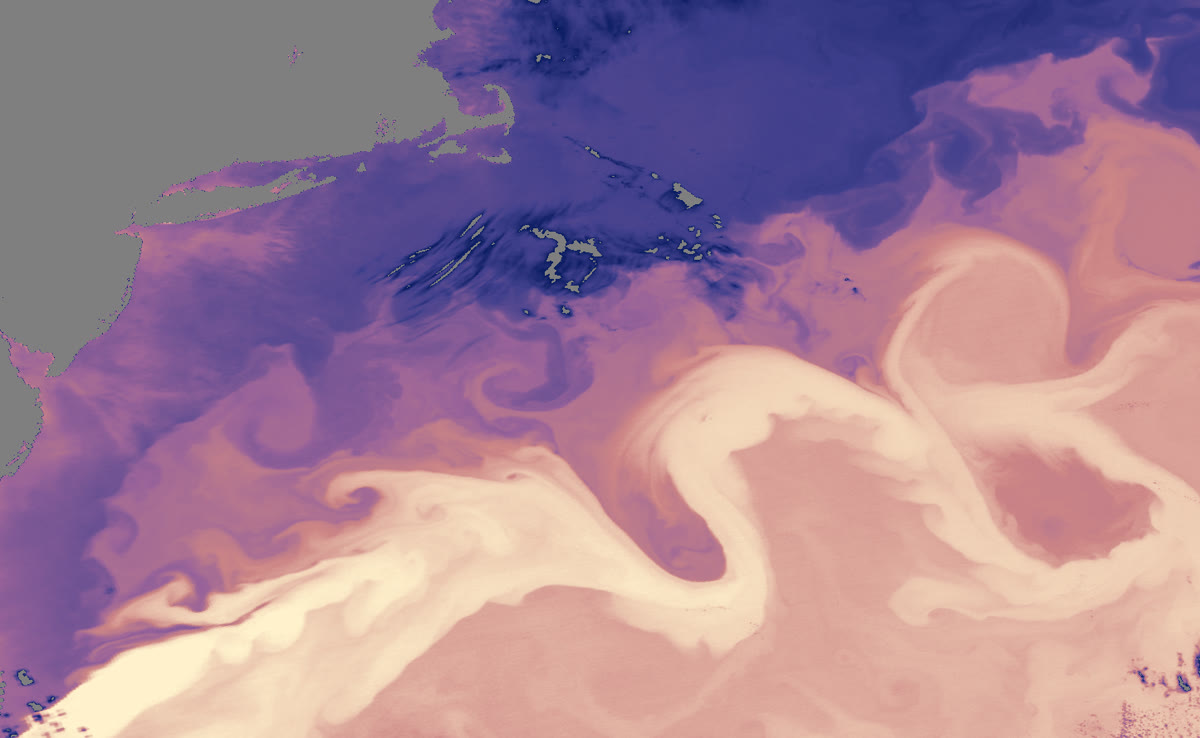
\includegraphics[width=\linewidth]{images/book1/g8-gulf-stream-sst.jpg}
\end{minipage}\hfill
\begin{minipage}[c]{0.46\linewidth}\raggedright
{\small La température de la surface de la \omterm{def:g2:water-on-earth:ocean}{mer} au large de la \omterm{def:g1:landscapes-around-us:water}{côte} est de
l'Amérique du Nord, mesurée par le satellite Aqua de la NASA le 18~avril
2005. Le Gulf Stream est la bande d'eau chaude (couleurs claires, jusqu'à
environ \qty{23}{\degreeCelsius}) qui serpente du bas à gauche vers la
droite, entre des eaux plus froides (sombres, jusqu'à environ
\qty{-1}{\degreeCelsius})~; les terres sont en gris. NASA (domaine public,
via Wikimedia Commons).}
\end{minipage}
% ledger: commons:gulf-sst
\label{fig:g8:the-oceans:gulf}
\end{omfigure}


\section{Les courants profonds et la chaleur de l'océan}

Les vents entraînent les courants de surface. Bien plus bas, dans
l'obscurité froide de l'\omterm{def:g2:water-on-earth:ocean}{océan} profond, l'eau bouge aussi, beaucoup plus lentement. Dans le
nord de l'Atlantique Nord, l'eau chaude apportée par le Gulf Stream cède
sa chaleur à l'air froid~; refroidie, et rendue plus salée quand la
banquise se forme, elle devient plus dense et coule jusqu'au fond. Cette
eau froide et salée se glisse vers le sud le long du fond de l'\omterm{def:g2:water-on-earth:ocean}{océan},
jusqu'à l'Antarctique, puis dans les \omterm{def:g2:water-on-earth:ocean}{océans} Indien et Pacifique, où elle
remonte lentement et revient en surface. Une goutte d'eau peut mettre
environ \num{1000}~ans à faire une fois le tour de cette grande boucle, le
\emph{tapis roulant océanique mondial}.
% ledger: nos:conveyor, nos:sea-ice-salt

\begin{omfigure}
\begin{tikzpicture}
\begin{axis}[ommap, width=\linewidth, xmin=-180, xmax=180, ymin=-65, ymax=70,
  xtick={-180,-120,...,180}, ytick={-60,-30,0,30,60},
  xticklabels={$180^\circ$,$120^\circ$O,$60^\circ$O,$0^\circ$,$60^\circ$E,$120^\circ$E,$180^\circ$},
  yticklabels={$60^\circ$S,$30^\circ$S,$0^\circ$,$30^\circ$N,$60^\circ$N},
  tick label style={font=\scriptsize}]
  \addplot[fill=omLithAlluv, draw=black!45, line width=0.2pt] table {figdata/out/shared-geo-land.dat};
  \addplot[omWarm, line width=1.3pt] table {figdata/out/grade-8-conveyor-surface.dat};
  \addplot[omCold, line width=1.3pt, dashed] table {figdata/out/grade-8-conveyor-deep.dat};
  \addplot[quiver={u=\thisrow{u}, v=\thisrow{v}}, -{Stealth[length=2.6mm, width=2.2mm]}, omWarm, line width=1.3pt]
    table[x=lon, y=lat] {figdata/out/grade-8-conveyor-heads-surface.dat};
  \addplot[quiver={u=\thisrow{u}, v=\thisrow{v}}, -{Stealth[length=2.6mm, width=2.2mm]}, omCold, line width=1.3pt]
    table[x=lon, y=lat] {figdata/out/grade-8-conveyor-heads-deep.dat};
  \node[font=\scriptsize\bfseries, fill=white, inner sep=1pt, anchor=west] at (axis cs:4,64) {plonge};
  \node[font=\scriptsize\bfseries, fill=white, inner sep=1pt, anchor=south] at (axis cs:163,11) {remonte};
\end{axis}
\end{tikzpicture}

{\small Le tapis roulant océanique mondial, simplifié en une seule boucle
(un croquis). En rouge~: l'eau chaude de surface~; en bleu, en tirets~:
l'eau froide et salée qui se glisse le long du fond de l'\omterm{def:g2:water-on-earth:ocean}{océan} profond.
L'eau plonge dans le nord de l'Atlantique Nord, entre le Groenland et la
Norvège, et remonte dans le Pacifique (et, non dessiné, dans l'\omterm{def:g2:water-on-earth:ocean}{océan}
Indien).}
% ledger: nos:conveyor, data:ne-land (figdata/grade-8/conveyor.py)
\end{omfigure}

\begin{example}[À quelle lenteur va l'eau profonde~?]\label{ex:g8:the-oceans:deep-speed}
La boucle dessinée sur la \omterm{def:g2:drawing-to-map:map}{carte} mesure environ \qty{70000}{km}. Si une
goutte d'eau met environ \num{1000}~ans à en faire le tour, elle avance en
moyenne d'environ $\num{70000} \div \num{1000} = \qty{70}{km}$ par an, soit
environ \qty{200}{m} par jour. Le Gulf Stream, à \qty{6.4}{km} à l'heure,
parcourt environ \qty{150}{km} en un jour~: il va aussi loin en environ
11~heures que l'eau profonde en une année entière.
% ledger: nos:conveyor, nos:gulf-stream, earth:Rmean (loop length and speeds computed in figdata/grade-8/conveyor.py)
\end{example}

Ensemble, les courants de surface et les courants profonds transportent de
la chaleur~: l'eau chaude va des \omterm{def:g5:weather-and-climate:tropics}{tropiques} vers les \omterm{def:g3:continents-and-oceans:poles}{pôles}, et l'eau froide
revient vers l'\omterm{def:g3:continents-and-oceans:equator}{équateur}. Comme les vents, l'\omterm{def:g2:water-on-earth:ocean}{océan} compense le chauffage
inégal de la Terre par le Soleil.
% ledger: nos:conveyor, nos:gulf-stream, mo:global-circ

\section{Exercices}

\begin{exercise}[$\star$]\label{exo:g8:the-oceans:1}
Range ces parties du fond de l'\omterm{def:g2:water-on-earth:ocean}{océan} dans l'ordre où un sous-marin les
rencontre en quittant une \omterm{def:g1:landscapes-around-us:water}{côte} pour le milieu de l'Atlantique~: \omterm{def:g8:the-oceans:seafloor}{plaine
abyssale}~; \omterm{def:g8:the-oceans:seafloor}{talus continental}~; \omterm{def:g8:the-oceans:seafloor}{dorsale océanique}~; \omterm{def:g8:the-oceans:seafloor}{plateau continental}.
\end{exercise}

\begin{exercise}[$\star$]\label{exo:g8:the-oceans:2}
Vrai ou faux~? Corrige les phrases fausses. (a) L'\omterm{def:g2:water-on-earth:ocean}{océan} a une profondeur
moyenne d'environ \qty{37}{km}. (b) Les \omterm{def:g8:the-oceans:current}{gyres} de l'\omterm{def:g3:continents-and-oceans:equator}{hémisphère} Nord tournent
dans le sens des aiguilles d'une montre. (c) L'évaporation rend l'eau de
\omterm{def:g2:water-on-earth:ocean}{mer} moins salée. (d) Le Gulf Stream est un courant chaud.
\end{exercise}

\begin{exercise}[$\star$]\label{exo:g8:the-oceans:3}
Donne le mot qui correspond à chaque description~: (a) une longue \omterm{def:g4:world-physical-map:range}{chaîne
de montagnes} sous la \omterm{def:g2:water-on-earth:ocean}{mer}~; (b) la masse de sel dans un kilogramme d'eau de
\omterm{def:g2:water-on-earth:ocean}{mer}~; (c) une très grande boucle de \omterm{def:g8:the-oceans:current}{courants océaniques}~; (d) un sillon
long, étroit et très profond du fond de l'\omterm{def:g2:water-on-earth:ocean}{océan}.
\end{exercise}

\begin{exercise}[$\star$]\label{exo:g8:the-oceans:4}
Sur la \omterm{def:g2:drawing-to-map:map}{carte} des \omterm{def:g8:the-oceans:current}{gyres}~: (a) dans quel sens tourne le \omterm{def:g8:the-oceans:current}{gyre} de
l'Atlantique Sud~? (b) Nomme un courant chaud et un courant froid de
l'Atlantique Nord. (c) Quels vents poussent l'eau vers l'ouest près de
l'\omterm{def:g3:continents-and-oceans:equator}{équateur}~?
\end{exercise}

\begin{exercise}[$\star\star$]\label{exo:g8:the-oceans:5}
Un échantillon de \qty{1}{kg} d'eau de \omterm{def:g2:water-on-earth:ocean}{mer} contient \qty{35}{g} de sels.
(a) Quel pourcentage de sa masse est du sel~? (b) Combien de grammes de
sels y a-t-il dans \qty{20}{kg} de cette eau~? (c) Combien de kilogrammes
d'eau de \omterm{def:g2:water-on-earth:ocean}{mer} contiennent \qty{1}{kg} de sels~?
\end{exercise}

\begin{exercise}[$\star\star$]\label{exo:g8:the-oceans:6}
Le sonar d'un navire envoie une impulsion sonore droit vers le bas. L'écho
revient \qty{6}{s} plus tard. Le son parcourt environ \qty{1500}{m} par
seconde dans l'eau de \omterm{def:g2:water-on-earth:ocean}{mer}. (a) Quelle distance le son parcourt-il en
\qty{6}{s}~? (b) Pourquoi la profondeur n'est-elle que la moitié de cette
distance~? (c) Quelle est la profondeur~? (d) Au-dessus de quelle partie
du fond de l'\omterm{def:g2:water-on-earth:ocean}{océan} le navire pourrait-il se trouver~?
\end{exercise}

\begin{exercise}[$\star\star$]\label{exo:g8:the-oceans:7}
Utilise le profil à travers l'Atlantique Sud. (a) Quelle est à peu près
la profondeur des \omterm{def:g8:the-oceans:seafloor}{plaines abyssales}~? (b) À quelle distance le long du
profil se trouve la crête de la dorsale médio-atlantique, et quelle est
sa profondeur~? (c) De combien de mètres la dorsale s'élève-t-elle
au-dessus des \omterm{def:g1:landscapes-around-us:landform}{plaines}~? (d) Pourquoi le profil a-t-il besoin d'une
exagération verticale~?
\end{exercise}

\begin{exercise}[$\star\star$]\label{exo:g8:the-oceans:8}
La \omterm{def:g2:water-on-earth:ocean}{mer} A se trouve entre deux \omterm{def:g5:weather-and-climate:desert}{déserts}~: il n'y pleut presque jamais et
aucun grand fleuve ne s'y jette. La \omterm{def:g2:water-on-earth:ocean}{mer} B, dans une région pluvieuse,
reçoit de nombreux grands fleuves. Explique laquelle des deux est plus
salée que l'\omterm{def:g2:water-on-earth:ocean}{océan} ouvert, et laquelle l'est moins. Utilise les mots
\emph{évaporation}, \emph{\omterm{def:g2:water-on-earth:salt-fresh}{eau douce}}, \emph{les sels restent}.
\end{exercise}

\begin{exercise}[$\star\star$]\label{exo:g8:the-oceans:9}
Un message dans une bouteille est jeté à la \omterm{def:g2:water-on-earth:ocean}{mer} au large de la \omterm{def:g1:landscapes-around-us:water}{côte} de la
Floride. (a) Quel courant l'emporte d'abord, et dans quelle direction~?
(b) Dans quel sens traverse-t-il ensuite l'Atlantique~? (c) S'il
continuait le tour du \omterm{def:g8:the-oceans:current}{gyre}, le long de quelle \omterm{def:g1:landscapes-around-us:water}{côte} descendrait-il vers le
sud~? (d) Ce courant est-il chaud ou froid~?
\end{exercise}

\begin{exercise}[$\star\star$]\label{exo:g8:the-oceans:10}
Le Gulf Stream avance en moyenne à environ \qty{6.4}{km} par heure. (a)
Quelle distance son eau parcourt-elle en un jour~? (b) En une semaine~?
(c) Compare avec une personne qui marche à \qty{5}{km} par heure.
\end{exercise}

\begin{exercise}[$\star\star\star$]\label{exo:g8:the-oceans:11}
L'\omterm{def:g2:water-on-earth:ocean}{océan} a une profondeur moyenne d'environ \qty{3700}{m}, et son point le
plus profond se trouve à près de \qty{11000}{m}. (a) Écris les deux
profondeurs en kilomètres. (b) Combien de fois le point le plus profond
est-il plus profond que la moyenne~? Arrondis au dixième. (c) Un écho de
sonar renvoyé par le point le plus profond~: combien de secondes met-il à
revenir, à \qty{1500}{m} par seconde~? (d) Une goutte d'eau du tapis
roulant plonge dans l'Atlantique Nord. Si elle met environ \num{1000}~ans
à en faire le tour, combien d'années cela fait-il, en puissance de dix~?
\end{exercise}

\begin{exercise}[$\star\star\star$]\label{exo:g8:the-oceans:12}
Le grand tapis roulant de l'\omterm{def:g2:water-on-earth:ocean}{océan} profond commence en \omterm{def:g2:water-on-earth:ocean}{mer} de Norvège, au
large de la \omterm{def:g1:landscapes-around-us:water}{côte} norvégienne, là où l'eau chaude apportée par le Gulf
Stream cède sa chaleur à l'air froid. (a) À l'aide de la \omterm{def:g2:drawing-to-map:map}{carte} des \omterm{def:g8:the-oceans:current}{gyres}
et du chapitre, explique étape par étape comment cette eau chaude est
arrivée là depuis les \omterm{def:g5:weather-and-climate:tropics}{tropiques}, et quels vents l'ont poussée. (b)
Explique pourquoi l'eau plonge ensuite. (c) Où va-t-elle ensuite~?
\end{exercise}

\section{Problème~: Une bouée dérivante}

\begin{problem}[{Problème du week-end --- une bouée dérivante est lâchée au large
de la Floride et emportée autour du gyre de l'Atlantique Nord~; son
voyage est suivi étape par étape, et l'on calcule le temps qu'il lui faut
pour en faire une fois le tour}]
\label{pb:g8:the-oceans:1}
% ledger: nos:drifter, nos:gulf-stream, nos:gyres (figdata/grade-8/ocean_currents.py; the leg lengths are rounded, the speeds of legs B to D are exercise data)
Des scientifiques lâchent une bouée dérivante au large de la \omterm{def:g1:landscapes-around-us:water}{côte} de la
Floride. Elle flotte juste sous la surface, se déplace avec les courants,
et envoie sa position à un satellite. Ses batteries durent environ un an.
La \omterm{def:g2:drawing-to-map:map}{carte} montre les quatre étapes de son voyage autour du \omterm{def:g8:the-oceans:current}{gyre} de
l'Atlantique Nord.

\begin{center}
\begin{tikzpicture}
\begin{axis}[ommap, width=11.5cm, xmin=-95, xmax=0, ymin=5, ymax=55,
  xtick={-90,-60,-30,0}, ytick={10,30,50},
  xticklabels={$90^\circ$O,$60^\circ$O,$30^\circ$O,$0^\circ$},
  yticklabels={$10^\circ$N,$30^\circ$N,$50^\circ$N},
  tick label style={font=\scriptsize}]
  \addplot[fill=omLithAlluv, draw=black!45, line width=0.2pt] table {figdata/out/shared-geo-land.dat};
  \addplot[black, line width=1pt, densely dashed, postaction={decorate, decoration={markings,
      mark=between positions 0.04 and 0.98 step 0.08 with {\arrow{Stealth[length=2mm]}}}}]
    table[x=lon, y=lat] {figdata/out/grade-8-ocean_currents-buoy.dat};
  \addplot[only marks, mark=*, mark size=2.2pt, omDef] coordinates {(-79.5,26)};
  \node[font=\scriptsize\bfseries, anchor=east, fill=white, inner sep=1pt] at (axis cs:-81,26) {lâcher};
  \addplot[only marks, mark=none, nodes near coords, point meta=explicit symbolic,
    every node near coord/.style={anchor=center, font=\footnotesize\bfseries, circle, fill=white, draw, inner sep=1pt}]
    table[x=lon, y=lat, meta=name] {figdata/out/grade-8-ocean_currents-buoy-legs.dat};
\end{axis}
\end{tikzpicture}

\medskip
{\small
\begin{tabular}{|c|l|c|c|}
\hline
étape & courant & longueur (km) & vitesse moyenne (km par jour) \\
\hline
A & Gulf Stream & 3800 & 100 \\
B & dérive nord-atlantique & 2100 & 20 \\
C & courant des Canaries & 3100 & 20 \\
D & courant nord-équatorial & 6100 & 20 \\
\hline
\end{tabular}}
\end{center}

\noindent\textbf{Partie I --- Le lâcher.}\par\nopagebreak
\begin{enumerate}[beginpenalty=10000]
  \item Dans quel \omterm{def:g2:water-on-earth:ocean}{océan}, et dans quel \omterm{def:g3:continents-and-oceans:equator}{hémisphère}, la bouée est-elle
        lâchée~?
  \item Dans quel sens tourne le \omterm{def:g8:the-oceans:current}{gyre}~? La bouée est-elle d'abord emportée
        vers le nord ou vers le sud~?
  \item L'eau de l'étape A est-elle chaude ou froide~? Et celle de
        l'étape C~? Explique.
  \item Quels vents entraînent les courants de l'étape B~? Ceux de
        l'étape D~?
\end{enumerate}

\noindent\textbf{Partie II --- Autour du gyre.}\par\nopagebreak
\begin{enumerate}[resume, beginpenalty=10000]
  \item Combien de jours dure l'étape A~?
  \item Combien de jours durent les étapes B, C et D~?
  \item Quelle est la longueur totale du voyage autour du \omterm{def:g8:the-oceans:current}{gyre}~?
  \item Pourquoi l'étape A est-elle tellement plus rapide que les autres~?
\end{enumerate}

\noindent\textbf{Partie III --- La durée du voyage.}\par\nopagebreak
\begin{enumerate}[resume, beginpenalty=10000]
  \item Combien de jours faut-il à la bouée pour faire une fois le tour du
        \omterm{def:g8:the-oceans:current}{gyre}~?
  \item En comptant un mois pour 30~jours, combien de mois cela fait-il~?
        Arrondis au mois près.
  \item Sur quelle étape les batteries seront-elles épuisées, au bout
        d'environ un an (365~jours)~?
  \item De combien de mois de batterie supplémentaires la bouée aurait-elle
        besoin pour envoyer sa position pendant tout le tour~?
\end{enumerate}
\end{problem}
